\chapter{Background}
\label{ch:background}
Recommender systems create opportunities and challenges for industry to understand consumption behaviour of users. In particular, for music industry, the development of recommender systems could improve digital music sales \parencite{ringen_2015}, and also, it could assist the listeners to discover new music through their habits \parencite{1_hypebot.com_2015}. However, when there is no priori information of a new introduced item in a recommender system, known as the \textit{cold-start problem}, popular songs could be favoured in recommendation process instead of items in the \textit{long tail}, i.e., songs that do not have enough ratings. Usually, content-based recommender systems are used to solve the cold-start problem because similarities between items are based on the content without regarding the ratings \parencite{Park200811}. Another solution to address the cold-start problem is to combine recommendation techniques to boost the strengths of each technique in an hybrid architecture. \parencite{melville2010recommender}

In this chapter, we present the importance of online social networks and music services platforms for retrieving user-item information, in conjunction with related work on music recommender systems. Subsequently, a novel approach of an hybrid recommendation model based on estimation of distribution algorithms (EDAs) is introduced and examined.

\section{Online Social Networks}
Social network sites \parencite{JCC4:JCC4393} are defined as: \begin{quote}``Web-based services that allow individuals to (1) construct a public or semi-public profile within a bounded system, (2) articulate a list of other users with whom they share a connection, and (3) view and traverse their list of connections and those made by others within the system.''\end{quote}

During the last decade, online social networks, which are also identified as \textit{social media} platforms, have become the outstanding technologies for retrieving and exchanging multimedia information \parencite{Putzke2014519}. Facebook, Twitter or YouTube, have enabled users to produce and share content on the internet, specially, customers around the world are renovating business models by sharing reviews and comments of products directly to companies. This produced content provides opportunities for research to track consumer's behaviour. \parencite{smith2009social}

In particular, Last.fm\footnote{http://www.last.fm/} is an online radio station that also have the facilities of a social media platform, where a user profile is built up by collecting the music tracks listened on multimedia players through a indexing process called \emph{scrobbling}. This profile may expose music consumption and listening behaviour. \parencite{Putzke2014519}

%\subsection{Last.fm}
\section{Music services platforms}
\label{sec:musicservices}
The Echo Nest\footnote{http://developer.echonest.com/} was a music intelligence company that offered solutions for music discovery and personalisation, dynamic curated sources, audio fingerprinting and interactive music applications. In 2014, The Echo Nest was acquired by Spotify\footnote{https://www.spotify.com/}, which is a commercial music streaming service, where a user can browse and listen music tracks sorted by artists, albums, genres or playlists. 

However, The Echo Nest API is still active for developer community and offers the access to artists, songs, taste profiles and playlists data. Particularly, The Echo Nest API is able to retrieve information limited to a particular music tracks catalogue such as 7digital\footnote{http://developer.7digital.com/}.

Both The Echo Nest and 7digital require to sign up for a free account to get unique keys for OAuth\footnote{http://oauth.net/} authentication in order to retrieve desired information through their respective APIs. As well, free account has limited number of calls, in the case of Echo Nest is limited to 20 request per minute and in the case of 7digital is limited to 4000 request per day.

In this project, we use a The Echo Nest account to get music tracks identifiers for each song in the user-item dataset and we use a 7digital developer account to fetch audio for each music track catalogue identifier. The user-item dataset consist of user - song - play count triplets of the Taste Profile\footnote{http://labrosa.ee.columbia.edu/millionsong/tasteprofile} subset which contains real world listeners activity provided among Echo Nest partners including Last.fm.
%\subsection{7Digital}
%\subsection{APIs}
%The publicly available music related information can be collected from user profiles on social networks using Application Program Interface (API).
%\section{Data Fusion Techniques}
%Combination of multiple sources of information to obtain more relevant parameters is known as data fusion.
%In this study, a cooperative data fusion technique is considered to augment information provided from social network source to content-based system features. \citep{Castanedo2013}

\section{Recommender Systems}
Recommender systems are software or technical facilities to provide items suggestions or predict customer preferences by using prior user information. These systems play an important role in commercial applications to increase sales and convey user satisfaction. In general, recommender systems can be categorised in two major groups: collaborative filtering and content-based filtering \parencite{melville2010recommender}.

\textcite{1242} considers also another methods for music recommendation such as \textit{demographic filtering} and \textit{named context-based}.

\subsection{Collaborative filtering}
In collaborative filtering (CF) \parencite{Yao2015453}, a \emph{m$\times$n} rating matrix (Figure~\ref{fig:useritemmatrix}) represents the relationships between \textit{m} users and \textit{n} items.
\begin{figure}[ht!]
	\centering
	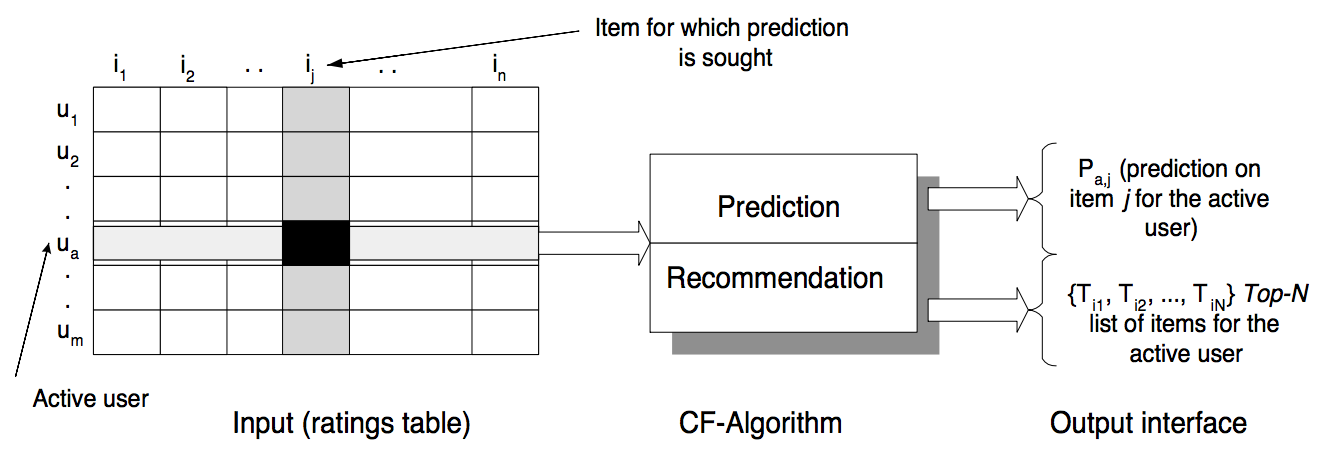
\includegraphics[width=\textwidth]{chapter2/user_item_data.png}
	\caption{Collaborative filtering process \parencite{sarwar2001item}}
	\label{fig:useritemmatrix}
\end{figure}

Recommendations are based on the computed similarities between rows (for users) or columns (for items), hence, CF can be further subdivided in the following neighbourhood models \parencite{Hu2008263}:

\begin{itemize}
	\item \textbf{User based} collaborative filtering, produce a recommendation of a previously unseen item based on similarity between users (Figure~\ref{fig:userbasedcf}).

	\begin{figure}[h!]
		\centering
		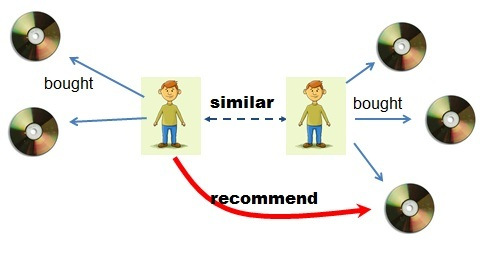
\includegraphics[width=0.5\textwidth]{chapter2/user-user1.jpg}
		\caption{User based collaborative filtering \parencite{1_siddharths_blog_2013}}
		\label{fig:userbasedcf}
	\end{figure}
	
	\item \textbf{Item based} collaborative filtering, produce a recommendation by comparing the similarities between a previously unseen item and the user's items (Figure ~\ref{fig:itembasedcf}).
	
	\begin{figure}[ht!]
		\centering
		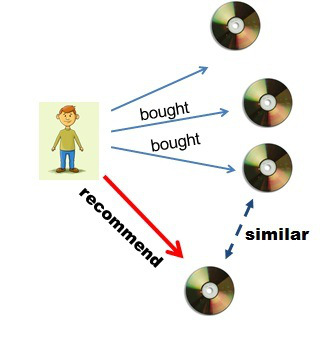
\includegraphics[width=0.4\textwidth]{chapter2/item-item1.jpg}
		\caption{Item based collaborative filtering \parencite{1_siddharths_blog_2013}}
		\label{fig:itembasedcf}
	\end{figure}
	
\end{itemize}

Similarities between a pair of users \emph{a,u} are usually computed with Pearson correlation metric \parencite{sarwar2001item}, given by Equation~\eqref{eq:pearson}:
\begin{equation}
	sim(a,u) =\frac{\sum _{i\in I}(r_{a,i} - \bar{r}_a)(r_{u,i} - \bar{r}_u)}{\sqrt{\sum _{i\in I}(r_{a,i} - \bar{r}_a)^2} \sqrt{\sum _{i\in I}(r_{u,i} - \bar{r}_u)^2}}
	\label{eq:pearson}
\end{equation}
where \emph{I} is the set of items rated by both users, $r_{u,i}$ is the rating given to item \emph{i} by user \emph{u}, and $\bar{r}_u$ is the mean rating given by user \emph{u}. Equivalently, for similarities between a pair of items \emph{i,j}, the correlation is given by Equation~\eqref{eq:pearson2}:
\begin{equation}
sim(i,j) =\frac{\sum _{u\in U}(r_{u,i} - \bar{r}_i)(r_{u,j} - \bar{r}_j)}{\sqrt{\sum _{u\in U}(r_{u,i} - \bar{r}_i)^2} \sqrt{\sum _{u\in U}(r_{u,j} - \bar{r}_j)^2}}
\label{eq:pearson2}
\end{equation}
where \emph{U} is the set of users who have rated both items, $r_{u,i}$ is the rating given to item \emph{i} by user \emph{u}, and $\bar{r}_i$ is the mean rating given to item \emph{i}.

The strength of CF is that the recommendation process is independent of the item features \parencite{Burke2002331}. On the other hand, CF would not be suitable technique when the user-item matrix is sparse. Moreover, CF considers only the most rated items, therefore, ignores the items in the long tail, and it is unable to handle the cold start problem. \parencite{Dai20141760}

\subsubsection{The cold start problem}
Recommendation process in CF might be difficult either for a user or an item with few ratings. \parencite{Burke2002331}

\subsubsection{The long tail phenomenon}
The \textit{long tail} items according to \textcite{Yin2012896} are referred to products with a low volume of sales but they can be more profitable than the popular items if they are recommended to the right consumers.

\subsection{Content-based filtering}
Content based (CB) filtering is based on the analysis of the features that describe the items. The recommendation component consists in matching up the attributes of the items that a user has already rated, usually referred as the \textit{user profile} \parencite{Lops2011}, against the attributes of a previously unseen products to produce a list of \emph{top-N} recommendations. Figure~\ref{fig:cb} shows the architecture of content-based recommendation process.
\begin{figure}[ht!]
	\centering
	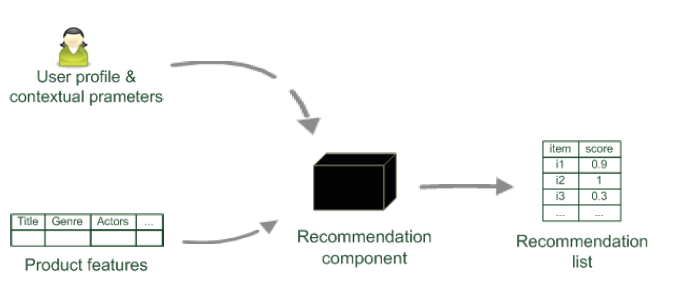
\includegraphics[width=0.8\textwidth]{chapter2/content-based-recommender1.png}
	\caption{Content-based filtering process \parencite{1_blogseagatesoftcom_2015}}
	\label{fig:cb}
\end{figure}

One of the strengths of CB filtering is that recommendation process is entirely based on the attributes of the items, thus, the recommendations produced for each user is independent from the other users information. Also, a CB recommender allows to recommend items that do not have any ratings, therefore, they can diminish the effects of cold-start problem. \parencite{Lops2011}

\subsubsection{Limitations of CB filtering}
One disadvantage of CB filtering is that personal reviews are not considered in the recommendation process, because this technique is limited to explicit representation of items~\parencite{1242}. Moreover, some representations limit the description to certain aspects only~\parencite{Lops2011}.

Another limitation of CB might be the collection of external data due to restricted access, e.g., the Million Song Dataset \parencite{Bertin-Mahieux2011} does not provide audio data due to copyright restrictions\footnote{http://labrosa.ee.columbia.edu/millionsong/pages/can-i-contact-you-privately-get-audio} and some preview clips are not available in the 7digital UK music catalogue. 

In our project, a CB recommender is used as the baseline to show a improved performance in music recommendation. Please refer to Section~\ref{sec:recresults} for more detail.

\subsection{Item Representation}
Items require an accurate description to achieve upstanding results for recommending items to users~\Autocite{1242}. In majority of the content-based filtering systems, item attributes are textual features extracted from web resources.~\parencite{Lops2011}

In our approach, we describe the songs in terms of n-dimensional vectors. Each dimension in the vector represent the probability of the song to belong to a music genre. The probalitity estimation is obtained from a music classifier implemented with a deep learning technique. The song representation process is illustrated in section~\ref{subsec:genre}

\subsection{User Modelling}
``User modeling [sic] is a discipline that deals with both how information about the user can be acquired and used by an automated system.''~\parencite{recsys2012}

Modelling a user profile consists of designing a structure for recording the interests which describe a user. There are several techniques for modelling an user profiles: vector, connexion, ontology and multidimensional representation. \parencite{DBLP:journals/corr/abs-1305-1114}

In our project, we model each user profile through EDAs by minimising a fitness function. The parameters of the fitness function are the rating and similarity values of each song that a user has listened. The user profile is also represented in a n-dimensional vector of probabilities of music genres. This process is illustrated in section~\ref{subsec:profile}

\subsection{Hybrid recommender approaches}
\label{subsec:hybridrecommender}
An hybrid recommender system is developed through the combination of the recommendation techniques mentioned in the previous sections. Usually, hybrid approaches boost the advantages of CF by considering the user's feedback and the advantages of CB by taking into count the item attributes.

According to \textcite{Burke2002331}, there are the following combination methods to accomplish hybridisation:
\begin{itemize}
	\item \textbf{Weighted} method, where a single item recommendation is computed as a linear combination of the recommendation value from each technique involved. The weight assigned to each recommender can be adjusted by considering additional feedback from the user.
	\item \textbf{Switching} method, where the hybrid system uses a criteria depending on the input data to switch between recommendation techniques implemented in the system.
	\item \textbf{Mixed} method, where recommendations from several different types of recommender are presented simultaneously.
	\item \textbf{Feature combination} method, where CF results are treated as additional attributes of a CB filtering recommender.
	\item \textbf{Cascade} method, where one recommender refines the coarse recommendations set given by the first recommender. This method is more efficient than the weighted method, because cascade implementation do not process every item at each stage.
	\item \textbf{Feature augmentation} method, where the rating of an item from one recommender is used as an input feature of another recommendation technique.
	\item \textbf{Meta-level} method, where a model generated for user's interest representation using one recommendation technique is used as the input of another recommender system. The advantage of this method is the performance of the second recommender that uses the compressed representation instead of sparse raw data.
\end{itemize}

The hybrid music recommender approach in this project can be considered as implementation of feature augmentation method and a meta-level method. The general model of our hybrid recommender is explained in detail in Section~\ref{sec:algorithms}.

%is based on a three-way aspect model \citep{Yoshii2008435}. Real item ratings are obtained through Last.fm API and spectral information are represented by convolutional deep belief networks (CDBN) features computed from items' spectrogram \citep{Lee20091096}.

\section{Music Information Retrieval}
Music Information Retrieval (MIR) \parencite{Casey2008668} is a field of research for better human understanding of music data in an effort to reduce the \textit{semantic gap} \parencite{Celma2006} between high-level musical information and low-level audio data. Applications of MIR include artist identification, genre classification and music recommender systems~\parencite{weston2012latent,Yoshii2008435}.

\subsection{Genre classification}
Music classification is one of the main tasks in MIR for clustering audio tracks based on similarities between features of pieces of music. Automatic musical genre classification approach proposed by \textcite{Tzanetakis2002293}, which uses GTZAN genre dataset\footnote{http://marsyas.info/downloads/datasets.html}, has been widely used in the past decade. The GTZAN dataset consists of a total of 1,000 clips, corresponding to 100 examples for each of the 10 music genres: blues, classical, country, disco, hiphop, jazz, metal, pop, reggae and rock. The total duration of each clip is 30 seconds.

Nonetheless, the GTZAN dataset has inaccuracies~\parencite{Sturm20127}, it still provides an useful baseline to compare genre classifiers.

\subsection{Music recommender systems}
\subsubsection{Collaborative retrieval music recommender}
\textcite{weston2012latent} proposed a latent \textit{collaborative retrieval} algorithm using the \textit{Last.fm Dataset - 1K users}\footnote{http://www.dtic.upf.edu/∼ocelma/MusicRecommendationDataset/lastfm-1K.html} dataset. For each (artist, song) tuplet in the dataset, they computed the audio data using 39-dimensional vector corresponding to 13 Mel Frequency Cepstral Coefficients (MFCCs),and the first and the second derivatives. The vectors obtained are used to build up a dictionary using the K-means algorithm. Each audio frame is represented with a vector that contains the number of occurrences of a dictionary vector in the frame. The collaborative retrieval algorithm present outperforming results compared with the Singular Value Decomposition (SVD) and Non-negative Matrix Factorization (NMF) methods used on collaborative filtering recommendation tasks. 

\subsubsection{Hybrid music recommender}
\textcite{Yoshii2008435} proposed a hybrid recommender system considering rating scores collected from Amazon.co.jp and acoustic features derived from the signals of musical pieces corresponding to Japanese CD singles that were ranked in weekly top-20 from April 2000 to December 2005. Acoustic features for each piece are represented as a \textit{bag-of-timbres}, i.e., a set of weights of polyphonic timbres, equivalent to a 13-dimensional MFCC representation. Bags of timbres are computed with a Gaussian Mixture Model, considering the same combination of Gaussians for all the pieces.

A three-way aspect model (see Figure~\ref{fig:threeway}) is used to decompose the joint probability of users \emph{U}, pieces \emph{M} and features \emph{T} into a set of latent genre variables \emph{Z}. It is assumed that user \emph{u} stochastically choose a genre \emph{z} according to their preferences and then the genre \emph{z} stochastically generates a piece of music \emph{m} and an acoustic feature \emph{t}.
\begin{figure}[ht!]
	\centering
	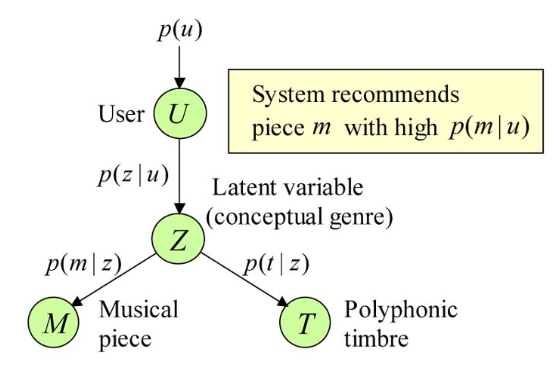
\includegraphics[width=0.5\textwidth]{chapter2/three_way_aspect_model.png}
	\caption{Three-way aspect model~\parencite{Yoshii2008435}}
	\label{fig:threeway}
\end{figure}

The results of the comparative experiments revealed that three-way aspect hybrid method outperformed the CF and CB recommendation techniques in terms of  accuracy considering $\vert T\vert=64$ features and $\vert Z\vert=10$ latent variables.

\section{Deep Learning}
High-level features that help us make sense of an observed data., e.g. genre, mood or release time in a music library could be difficult to compute. Deep learning algorithms allows us to build complex concepts out of simpler concepts \parencite{Bengio-et-al-2015-Book}. Deep learning can solve the difficulty of representing high-level features, e.g., perceived genre in a piece of music, by expressing them in terms of low-level signal features, e.g. spectrum, frequency or pitch.

In MIR, deep learning methods capture the attention of researchers for the following reasons~\parencite{kereliuk15}:
\begin{itemize}
	\item Hierarchical representations of structures in data.
	\item Efficient feature learning and classification algorithms.
	\item Open and publicly available implementations, e.g., \textit{Theano}~\parencite{Bastien-Theano-2012, bergstra+al:2010-scipy} library for Python.
\end{itemize}

These advantages of deep learning methods enable us to learn abstractions from music low-level content in order to reduce the \textit{semantic gap}~\parencite{Celma2006} in MIR. Additionally, feature extraction does not require significant domain knowledge compared to \textit{hand-crafted} engineering. Nonetheless, deep learning implementations require a lot of data.

\subsection{Deep Neural Networks}
A deep neural network (DNN) \parencite{hinton2012deep} is defined as a feed-forward artificial neural network (ANN), or multi-layer perceptron (MLP), with more than one layer of hidden units between the input and the output layer (see Figure~\ref{fig:dnn}).
\begin{figure}[ht!]
	\centering
	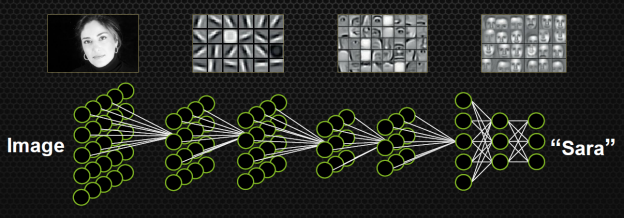
\includegraphics[width=\textwidth]{chapter2/dnn.png}
	\caption{Schematic representation of a deep neural network~\parencite{1_brown_2014}}
	\label{fig:dnn}
\end{figure}

Each hidden unit \emph{j} maps its total input from the layer below $x_j$, given by Equation~\eqref{eq:hiddenunit} 
\begin{equation}
x_j =b_j+\sum_{i}^{}y_iw_{ij}
\label{eq:hiddenunit}
\end{equation}
where $b_j$ is the bias of unit \emph{j}, \emph{i} is an index over units in the
layer below, and $w_{ij}$ is the weight on a connection to unit \emph{j}
from unit \emph{i} in the layer below, to a scalar value $y_j$ that is directed to the layer above. The activation function of hidden units can be hyperbolic tangent, logistic or rectifier linear activation function. For classification, output unit \emph{j} converts its total input $x_j$ into a class probability $p_j$ by using the \textit{softmax} nonlinearity, given by Equation~\eqref{eq:softmax}
\begin{equation}
p_j =\frac{\exp x_j}{\sum_{k}^{}\exp x_k}
\label{eq:softmax}
\end{equation}
where \emph{k} is the number of classes.
\subsubsection{Music Feature Learning}
\textcite{Sigtia20146959} examined and compared DNNs to discover features from the GTZAN dataset and the ISMIR 2004 genre classification dataset\footnote{http://ismir2004.ismir.net/genre\_contest/}, using rectifier linear units (ReLUs) and dropout regularisation. The ReLU activation function is defined as $max(x,0)$. ReLUs provides better convergence without pre-training. Dropout regularisation reduces the problem of overfitting.

First, the GTZAN dataset was divided into four 50/25/25 train, validation, test parts. For each audio clip of the dataset, they calculated the Fast Fourier Transform (FFT) on frames of length 1,024 samples (22,050 kHz sampling rate) with a window overlap of 50\%. Next, they used the magnitude of each FFT frame resulting in a 513 dimensional vector. And then, each feature dimension is normalised to have zero mean and unit standard deviation.

For the deep neural network, the 500 hidden units were trained with stochastic gradient descent (SGD) with a learning rate of 0.01, a patience of 10 and a dropout rate of 0.25.

The system classifies the GTZAN data with an accuracy of 83$\pm$1.1\%, a value of the same order of results obtained with hand-crafted features.

\subsection{Convolutional Deep Neural Networks}
Inspired in the behaviour of animal visual processing system~\parencite{1_deeplearning.net_2015}, a convolutional deep neural network (CDNN)~\parencite{Bengio-et-al-2015-Book, 1_ufldlstanfordedu_2015} is a type of MLP that uses convolution operation instead of matrix multiplication for processing data that has grid-like topology. CDNNs are designed to recognize visual patterns directly from pixel images. In general, the architecture of a CDNN is based on:
\begin{itemize}
	\item \textbf{Sparse connectivity:} the inputs of hidden units in an upper layer \emph{m} are from a subset of units in a lower layer \emph{m$-$1}.
	\item \textbf{Shared weights:} each hidden unit in a layer share the same weight vector and bias. The layer with this parametrisation form a \textit{feature map}.
	%\subitem To preserve the information about the input it is suggested to keeping the total number of activations (number of feature maps times number of pixel positions)
	\item \textbf{Convolutional layers:} A feature map is obtained by convolution of the input image with a linear filter, adding a bias term and then applying a non-linear function. Each convolutional (hidden) layer is composed of multiple feature maps.
	%\subitem The trick is thus to find the right level of “granularity” (i.e. filter shapes) in order to create abstractions at the proper scale, given a particular dataset.
	\item \textbf{Max-pooling:} is a non-linear down-sampling to divide the input image into a set of non-overlapping rectangles and, for each rectangle, the maximum value is returned.
	%Typical values are 2x2 or no max-pooling. Very large input images may warrant 4x4 pooling in the lower-layers.
\end{itemize}

LeNet-5~\parencite{1_lecun_2015} is one model of CDNN designed for recognition of handwritten and machine-printed characters. In Figure~\ref{fig:lenet}, the LeNet model is illustrated. The lower-layers are composed of convolution and max-pooling layers and the upper-layer is a fully-connected MLP. The input to MLP is the set of all features maps at the layer below.
\begin{figure}[ht!]
	\centering
	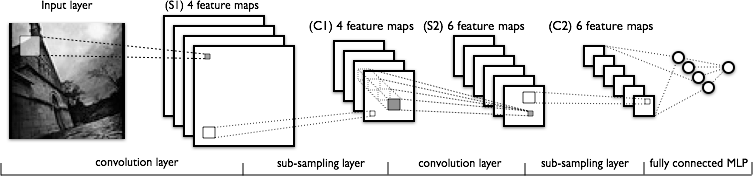
\includegraphics[width=1\textwidth]{chapter2/mylenet.png}
	\caption{Convolutional deep neural network LeNet model \parencite{1_deeplearning.net_2015}}
\label{fig:lenet}
\end{figure}

\subsubsection{Deep content-based music recommendation}
\textcite{NIPS2013_5004} proposed to use a latent factor model for CB recommendation and the implementation of a CDNN to predict the latent factors from music audio. To obtain 50-dimension latent vectors, they used a weighted matrix factorisation (WMF) algorithm on the Taste Profile Subset. Also, they retrieved audio clips for over 99\% of the songs in the dataset from 7digital.com.

To train the CDNN, the latent vectors obtained through the WMF are used as ground truth. The input of the CDNN is a log-compressed mel-spectrogram with 128 components computed from windows of 1,024 samples  and a hop size of 512 samples (sampling rate of 22,050 Hz) for each audio clip. The duration of audio clips is limited to 3 seconds.

They used 10-fold cross validation and obtained an average area under the ROC curve (AUC) of 0.86703 for prediction based on the latent factor vectors, outperforming the bag-of-timbres approach.

\section{Estimation of Distribution Algorithms}
Inspired in natural selection of species, an estimation of distribution algorithm (EDA) \parencite{pelikan2015estimation, Ding2015451, Santana:Bielza:Larrañaga:Lozano:Echegoyen:Mendiburu:Armañanzas:Shakya:2009:JSSOBK:v35i07} is an optimisation technique that estimates a probabilistic model from a sample of promising individuals, which is used to generate a new population and leading to an optimal solution of an objective function, called the \textit{fitness} function, until a termination criteria, e.g., maximisation, minimisation, maximum number of generations, is satisfied. These algorithms were applied to solve complex problems such as load balancing for mobile networks~\parencite{Hejazi15} or software reliability prediction~\parencite{Jin2014113}. In Figure~\ref{fig:eda} we show the general flowchart of an EDA.

\begin{figure}[ht!]
	\centering
	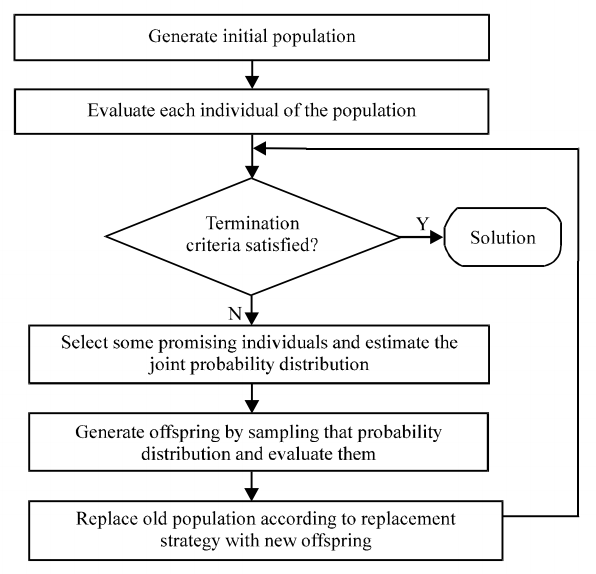
\includegraphics[width=0.5\textwidth]{chapter2/eda.png}
	\caption{Flowchart of estimation of distribution algorithm \parencite{Ding2015451}}
	\label{fig:eda}
\end{figure}

According to~\textcite{pelikan2015estimation}, the main components of an EDA are  a selection operator, a class of probabilistic models for modelling and sampling, and a replacement operator for combining the old population with the offspring. Also, regarding the types of distributions that an EDA are able to capture~\parencite{pelikan2015estimation} can be categorised in four broad groups: 
\begin{itemize}
	\item \textbf{Discrete variables EDAs}, where candidate solutions are represented by fixed-length strings of a finite cardinality.
	\item \textbf{Permutation EDAs}, where candidate solutions are represented by permutations over a given set of elements.
	\item \textbf{Real-valued vectors (continuous) EDAs}, where candidate solutions are mapped from real-valued variables into a discrete domain or the probabilistic model defined on real-valued variables are considered.
	\item \textbf{Genetic programming EDAs}.
\end{itemize}

The advantages of using EDAs include the discovery of problem-specific features or reducing the memory requirements. However, it is time consuming to build explicit probabilistic models.~\parencite{pelikan2015estimation}

In our project, we investigate permutation EDAs and continuous EDAs for user profile modelling.

\subsection{A Hybrid Recommendation Model Based on EDA}
\textcite{Liang2014781} exploited a permutation EDA to model user profiles in an hybrid model for movie recommendation using the MovieLens 1M dataset\footnote{http://grouplens.org/datasets/movielens/}.

A movie, \emph{i}, is described using a vector, $t_i=\{(k_1,w_1),\ldots ,(k_n,w_n)\}$, where the keywords $k_n$ and weights $w_n$ are calculated with term frequency-inverse document frequency (TF-IDF) technique. A user is initially represented by a set,  $S_u=\{(t_1, r_{u,1}),\ldots,(t_i, r_{u,i})\vert r_{u,i}>\bar r_{u}\}$, where, $r_{u,i}$ is the rating of the movie \emph{i} given by user \emph{u}, and $\bar r_{u}$ is a threshold. The keywords in every $S_u$ set are embedded in a new set, $D_u$.

The goal is to learn the user profile, $profile_u=\{(k_1,w_1),\ldots ,(k_n,w_n)\}$, by minimisation of the fitness function, defined by Equation~\eqref{eq:fitness}
\begin{equation}
fitness(profile_u) =\sum_{i\in S_u}\log(r_{u,i}\times sim(profile_u,t_i))
\label{eq:fitness}
\end{equation}
where $sim(profile_u,t_i)$ is computed by the cosine similarity coefficient, defined by Equation~\eqref{eq:cossim}
\begin{equation}
sim(profile_u, t_i)=cos(profile_u, t_i) =\frac{profile_u\cdot t_i}{\Vert profile_u\Vert\times\Vert t_i\Vert}
\label{eq:cossim}
\end{equation}

The pseudocode of EDA implemented by \textcite{Liang2014781} is delineated by Algorithm~\ref{alg:hybrideda}, where MAXGEN is the maximum number of generations.
\begin{algorithm}[ht!]
	\caption{Calculate $profile_u$}
	\begin{algorithmic} 
		\REQUIRE set $D_u$, weights $w_{n,i}$
		\REQUIRE population size $N$, MAXGEN
		%\ENSURE $y = x^n$
		\STATE Random selection of keywords $k_n$ from $D_u$
		\STATE Assign a weight $w_{n,i}$ to each $k_n$ to build a set~$K_u$ of size~$N$
		\STATE Assign a probability $c_{n,i}=1/N$ to each $(k_n,w_{n,i})$
		\STATE Generate initial population of $profile_u$ by Monte Carlo method
		\WHILE{$generation <$ MAXGEN}
		\STATE Compute each $fitness(profile_u)$
		\STATE Rank individuals by their fitness value
		\STATE Select top $M < N$ individuals
		\STATE Update $c_{n,i}$ by counting the occurrences of $(k_n,w_{n,i})$ in the $M$ individuals profiles
		\STATE Generate $profile_u$ by random sampling according to updated $c_{n,i}$
		\ENDWHILE
		\RETURN $profile_u$
	\end{algorithmic}
	\label{alg:hybrideda}
\end{algorithm}

To recommend a new movie, \emph{j}, to a user, the similarity between the user profile, $u_i$, and the movie vector, $t_j$, is calculated using Pearson correlation coefficient, defined by Equation~\eqref{eq:wpearson}:
\begin{equation}
sim(u_i,t_j) =\frac{\sum _{c\in I_i \cap I_j}^{ } (w_{i,c} - \bar{w}_i)(w_{j,c} - \bar{w}_j)}{\sqrt{\sum _{c\in I_u \cap I_j}^{ }(w_{i,c} - \bar{w}_i)^2} \sqrt{\sum _{c\in I_u \cap I_j}^{ }(w_{j,c} - \bar{w}_j)^2}}
\label{eq:wpearson}
\end{equation}
where, $c\in I_i \cap I_j$ are the keywords in common between the user profile and the new movie vector, $w_{i,c}$ and $w_{j,c}$ are the weights of keyword \emph{c} in the user profile and movie vector, $\bar{w}_i$ is the mean weight of user profile and $\bar{w}_j$ is the mean weight of movie vector.

In our approach, we use the algorithm proposed by~\textcite{Liang2014781} to model user profiles but considering probability values of music genres instead of weight values of keywords. The adapted algorithm is explained in subsection~\ref{subsec:profile}.

\subsection{Continuous Univariate Marginal Distribution Algorithm}

\textcite{gallagher2007bayesian} presented the continuous univariate marginal distribution algorithm ($UMDA_c^G$) as an extension of a discrete variable EDA. The general pseudocode of the $UMDA_c^G$ is delineated in Algorithm~\ref{alg:umda}, where $x_i\in \textbf{x}$ represent the \emph{i} parameter of \textbf{\emph{x}} individual solution.

\begin{algorithm}[ht!]
	\caption{Framework for $UMDA_c^G$}
	\begin{algorithmic} 
		\REQUIRE population size $M$
		\REQUIRE selection parameter $\tau$
		%\ENSURE $y = x^n$
		\STATE $t \leftarrow 0$
		\STATE Generate $M$ individuals at random
		\WHILE{$t <$ stopping criteria}
		\STATE $M_{sel}\leftarrow M\cdot\tau$
		\STATE Select $M_{sel}$ individuals 
		\STATE $\mu_{i,t}\leftarrow\frac{1}{M_{sel}}\sum_{j=1}^{M_{sel}}x_i^j$
		\STATE $\sigma_{i,t}^2\leftarrow\frac{1}{M_{sel}-1}\sum_{j=1}^{M_{sel}}(x_i^j-\mu_{i,t})^2$ 
		\STATE $p_t({x_{i}}\vert \mu_{i,t},\sigma_{i,t}^2)\leftarrow\frac{1}{\sqrt{2\pi}\sigma_{i,t}}\exp(-\frac{1}{2}(\frac{x_i-\mu_{i,t}}{\sigma_{i,t}})^2)$
		\STATE Sample $M$ individuals from $p_t({x_{i}}\vert \mu_{i,t},\sigma_{i,t}^2)$
		\STATE $t\leftarrow t+1$
		\ENDWHILE
	\end{algorithmic}
	\label{alg:umda}
\end{algorithm}

To our knowledge, our hybrid recommender design is the first work to consider a continuous EDA for user profile modelling in a recommender system. The implementation of the continuous EDA is explained in subsection~\ref{subsec:profile}.

\section{Summary}
In this chapter, previous work on recommender systems has been reviewed and novelty techniques to representing acoustical features and to model user profiles has been presented. The next steps are to collect the dataset by crawling online social information, to extract the acoustical features of a collection of songs to represent them as n-dimensional vectors, to model the user profiles by using EDAs, and therefore, to return a list of song recommendations.